% Provenance (never printed): cycle 4 SVT, "La planete Terre": the history of
% the Earth read in the rocks, relative dating (superposition, recoupement,
% inclusion, continuite paleontologique), the ages of the Earth, eras and
% periods, the scale of geological time; see sources/book1/PROVENANCE.md.
% Book 1, grade 7, chapter 5.
% Vocabulary guard: owns relative dating / absolute age, the four principles,
% unconformity, era and geological period, the geological time scale. The
% method of radiometric dating is the physics books' and grade 12's: told
% here in two sentences, never defined. Fossils as evidence of evolution are
% the biology books' (one sentence of prose). "Ice age" is grade 8's: not used.
\chapter{地球的年龄}\label{ch:g7:geological-time}

1788 年 6 月，苏格兰地质学家赫顿与两位朋友，
数学家普莱费尔和化学家霍尔，一同造访
锡卡尔角，一处被海水“冲刷得光秃秃”的\omterm{def:g3:stones-pebbles-sand:rock}{岩石}岬，位于苏格兰\omterm{def:g1:landscapes-around-us:water}{海岸}。
在\omterm{def:g3:stones-pebbles-sand:rock}{岩石}底部，他们看到灰色岩层直立着，
几乎竖直。其上覆盖着平缓倾斜的红色砂岩层。赫顿
解释了其中经过：灰色岩层先是水平\omterm{def:g5:water-shapes-the-land:deposition}{沉积}在
海底，随后被挤压抬升而直立，接着遭受\omterm{def:g5:water-shapes-the-land:erosion}{侵蚀}，然后
红色沙层才覆盖其上。这每一步都需要
极其漫长的时间。普莱费尔后来写道：“心智
似乎因凝望如此遥远的时间深渊而眩晕。”
% ledger: ncse:siccar-point

\begin{omfigure}
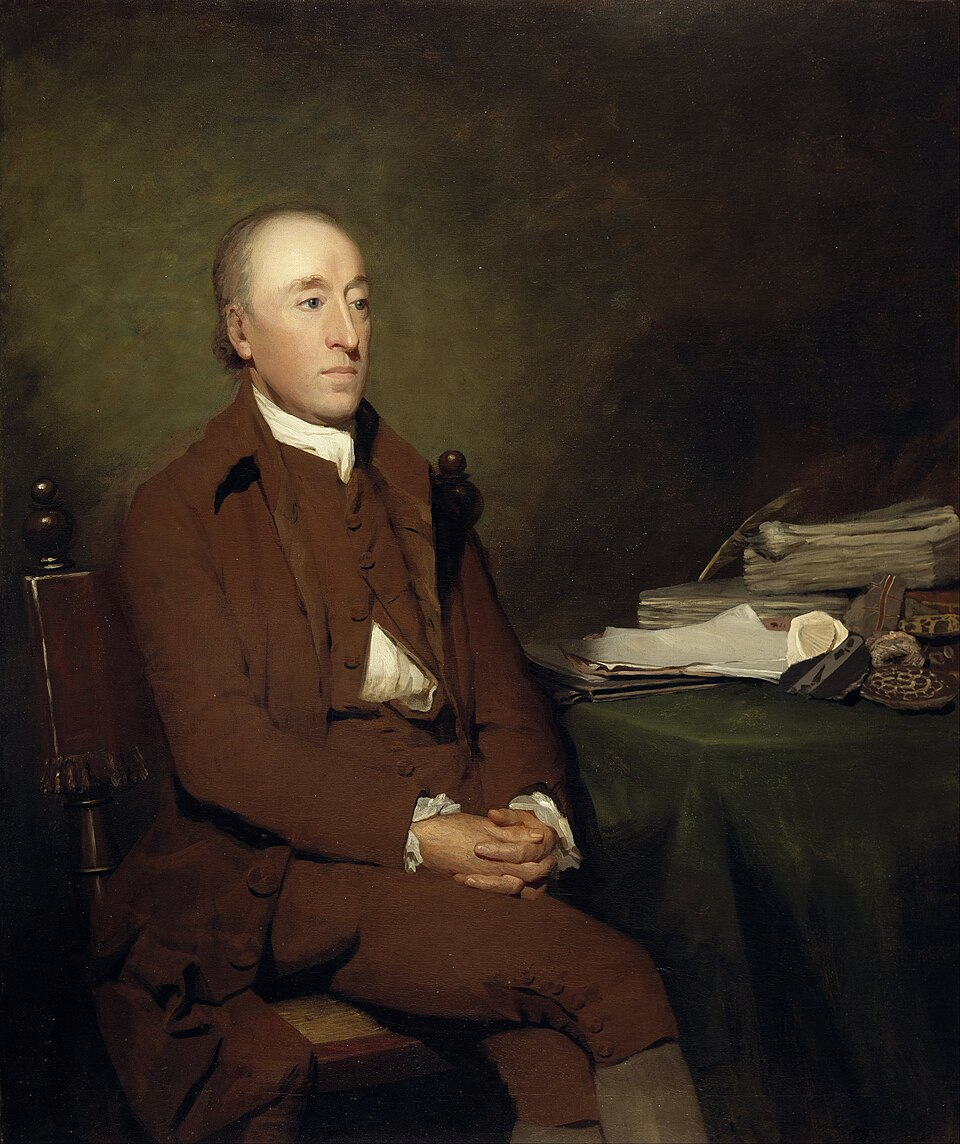
\includegraphics[width=0.3\linewidth]{images/book1/g7-hutton.jpg}

{\small 赫顿（1726--1797），Henry Raeburn 绘。
赫顿将每一层视为一段时间，最老的一层
总在最底部，只要岩层未被翻转。肖像属公有领域，经由维基
共享资源提供。}
% ledger: commons:hutton-portrait, usgs:hutton-smith
\label{fig:g7:geological-time:hutton}
\end{omfigure}

在没有任何日期标注的情况下，如何判断
一块\omterm{def:g3:stones-pebbles-sand:rock}{岩石}比另一块更老？地球究竟有多老？这样漫长的历史
又该如何描绘？

\begin{recall}
\omterm{def:g7:sediments-and-fossils:sediment}{沉积物}成层\omterm{def:g5:water-shapes-the-land:deposition}{沉积}，一层叠压在另一层之上，固结为
\omterm{def:g6:rocks-and-minerals:rock-families}{沉积岩}；\omterm{def:g7:sediments-and-fossils:fossil}{化石}是\omterm{def:g3:stones-pebbles-sand:rock}{岩石}中保存的生物遗体或遗迹
（见\cref{ch:g7:sediments-and-fossils}）。\emph{\omterm{def:g7:earthquakes:fault}{断层}}是
\omterm{def:g3:stones-pebbles-sand:rock}{岩石}中两侧发生过相对移动的断裂
（见\cref{ch:g7:earthquakes}）。花岗岩是一种\emph{\omterm{def:g6:rocks-and-minerals:rock-families}{火成岩}}，
由熔融\omterm{def:g3:stones-pebbles-sand:rock}{岩石}在地下深处缓慢冷却形成；片岩是一种
\emph{\omterm{def:g6:rocks-and-minerals:rock-families}{变质岩}}，由热和压力使\omterm{def:g3:stones-pebbles-sand:rock}{岩石}改变而成；砾岩是
一种由\omterm{def:g3:stones-pebbles-sand:pebble}{卵石}胶结而成的\omterm{def:g6:rocks-and-minerals:rock-families}{沉积岩}
（见\cref{ch:g6:rocks-and-minerals}）。
\end{recall}

\section{哪个先出现？}

历史学家即使没有日期，也能把事件排出先后。第一次世界大战
早于第二次世界大战，这从名称便可看出。电视机尚未进入
千家万户时，赖特兄弟已于 1903 年首次试飞，而许多
人在 1969 年通过电视看到了人类登上月球的第一步，因此
先有飞行，再有家庭电视，最后才是登月。收集
线索并加以比较，便足以确定先后。地球历史的
绝大部分时期都没有任何文字记录，地质学家
的工作方式与此相同：他们借助保存在\omterm{def:g3:stones-pebbles-sand:rock}{岩石}中的线索。
% ledger: usgs:events-order

\begin{definition}[相对定年与绝对年龄]\label{def:g7:geological-time:relative-dating}
\emph{相对定年}\index{相对定年}把\omterm{def:g3:stones-pebbles-sand:rock}{岩石}和事件按
先后排序，从最老排到最新，不说明距今多少年：
这块\omterm{def:g3:stones-pebbles-sand:rock}{岩石}比那块更老。
\emph{绝对年龄}\index{绝对年龄}是以年数给出的年龄，例如
“3 亿年”。
\end{definition}

\section{岩层排序的四条原理}

四条简单的原理承担了\omterm{def:g7:geological-time:relative-dating}{相对定年}的大部分工作。它们
如下图所示，画在四个想象中的悬崖上。第一条原理由斯泰诺于 1669 年提出，赫顿在十八世纪末以此为基础继续发展。
% ledger: usgs:hutton-smith, og:stratigraphy-principles

\begin{omfigure}
\tikzset{
  trilo/.pic={\fill[black!65] (0,0) ellipse (0.13 and 0.085);
              \draw[white, line width=0.3pt] (-0.11,0.028) -- (0.11,0.028) (-0.11,-0.028) -- (0.11,-0.028);},
  ammo/.pic={\draw[black!75, line width=0.45pt] (0,0) circle (0.1) (0,0) circle (0.062) (0,0) circle (0.028);}
}
\begin{minipage}[t]{0.49\linewidth}\centering
\begin{tikzpicture}[font=\footnotesize]
  \fill[lith sandstone] (0,0) rectangle (4.4,0.6);
  \fill[lith shale] (0,0.6) rectangle (4.4,1.2);
  \fill[lith limestone] (0,1.2) rectangle (4.4,1.8);
  \fill[lith sandstone] (0,1.8) rectangle (4.4,2.4);
  \foreach \k in {1,2,3,4} \node[fill=white, inner sep=1pt] at (0.35,0.6*\k-0.3) {\k};
  \draw (0,0) rectangle (4.4,2.4);
  \foreach \y in {0.6,1.2,1.8} \draw[contact] (0,\y) -- (4.4,\y);
  \draw[-{Stealth}, line width=0.8pt] (4.75,0.1) -- (4.75,2.3);
  \node[anchor=west] at (4.85,2.2) {最新};
  \node[anchor=west] at (4.85,0.2) {最老};
\end{tikzpicture}

{\small (a) \omterm{def:g7:geological-time:superposition}{叠加原理}：第 1 层最先形成，第 4 层最后形成。}
\end{minipage}\hfill
\begin{minipage}[t]{0.49\linewidth}\centering
\begin{tikzpicture}[font=\footnotesize]
  % left block, below the fault
  \begin{scope}
    \clip (0,0) -- (3.75,0) -- (3.25,2.4) -- (0,2.4) -- cycle;
    \fill[lith sandstone] (0,0) rectangle (5,0.6);
    \fill[lith shale] (0,0.6) rectangle (5,1.2);
    \fill[lith limestone] (0,1.2) rectangle (5,1.8);
    \fill[lith granite] (1.2,0) -- (1.85,0) -- (1.75,0.9) -- (1.9,1.8) -- (1.15,1.8) -- (1.3,0.9) -- cycle;
    \fill[lith sandstone] (0,1.8) rectangle (5,2.4);
    \foreach \y in {0.6,1.2} {\draw[contact] (0,\y) -- (1.25,\y); \draw[contact] (1.8,\y) -- (5,\y);}
    \draw[contact] (1.2,0) -- (1.3,0.9) -- (1.15,1.8) (1.85,0) -- (1.75,0.9) -- (1.9,1.8);
    \draw[contact] (0,1.8) -- (5,1.8);
  \end{scope}
  % right block, moved down along the fault
  \begin{scope}
    \clip (3.75,0) -- (5,0) -- (5,2.05) -- (3.32,2.05) -- cycle;
    \fill[lith sandstone] (3,-0.35) rectangle (5,0.25);
    \fill[lith shale] (3,0.25) rectangle (5,0.85);
    \fill[lith limestone] (3,0.85) rectangle (5,1.45);
    \fill[lith sandstone] (3,1.45) rectangle (5,2.05);
    \foreach \y in {0.25,0.85,1.45} \draw[contact] (3,\y) -- (5,\y);
  \end{scope}
  \draw (0,0) -- (5,0) -- (5,2.05) -- (3.32,2.05) (3.25,2.4) -- (0,2.4) -- (0,0);
  \draw[fault] (3.75,0) -- (3.25,2.4);
  \node[anchor=south, fill=white, inner sep=1pt] at (1.5,2.45) {花岗岩};
  \draw[black!70] (1.5,2.45) -- (1.52,1.6);
  \node[anchor=south] at (4.2,2.45) {断层};
  \draw[black!70] (4.0,2.45) -- (3.4,1.75);
\end{tikzpicture}

  {\small (b) \omterm{def:g7:geological-time:cross-cutting}{切割律}：花岗岩比它所切穿的三层岩层年轻，
比顶层岩层古老；\omterm{def:g7:earthquakes:fault}{断层}切断了所有岩层，
是最年轻的。}
\end{minipage}

\bigskip
\begin{minipage}[t]{0.49\linewidth}\centering
\begin{tikzpicture}[font=\footnotesize]
  \fill[lith granite] (0,0) -- (4.4,0) -- (4.4,1.05) .. controls (3.4,0.95) and (2.6,1.2) .. (1.6,1.0) .. controls (0.9,0.88) and (0.4,1.1) .. (0,1.0) -- cycle;
  \fill[lith conglomerate] (0,2.4) -- (4.4,2.4) -- (4.4,1.05) .. controls (3.4,0.95) and (2.6,1.2) .. (1.6,1.0) .. controls (0.9,0.88) and (0.4,1.1) .. (0,1.0) -- cycle;
  \foreach \x/\y/\a/\b in {0.5/1.35/0.2/0.12, 1.3/1.25/0.16/0.1, 2.1/1.45/0.22/0.13, 2.9/1.3/0.17/0.11, 3.7/1.4/0.2/0.12, 0.9/1.8/0.15/0.1, 2.5/1.95/0.17/0.1, 3.4/1.85/0.14/0.09}
    \filldraw[fill=omLithGranite, draw=black!70, line width=0.3pt] (\x,\y) ellipse [x radius=\a, y radius=\b];
  \draw[unconformity] (0,1.0) .. controls (0.4,1.1) and (0.9,0.88) .. (1.6,1.0) .. controls (2.6,1.2) and (3.4,0.95) .. (4.4,1.05);
  \draw (0,0) rectangle (4.4,2.4);
  \node[fill=white, inner sep=1pt] at (2.2,0.45) {花岗岩};
  \node[anchor=west] at (4.5,1.7) {砾岩};
  \node[anchor=west, align=left] at (4.5,1.15) {花岗岩 \\卵石};
  \draw[black!70] (4.5,1.15) -- (3.85,1.4);
\end{tikzpicture}

{\small (c) \omterm{def:g7:geological-time:inclusion}{包裹体律}：花岗岩\omterm{def:g3:stones-pebbles-sand:pebble}{卵石}比包裹它们的
砾岩古老。}
\end{minipage}\hfill
\begin{minipage}[t]{0.49\linewidth}\centering
\begin{tikzpicture}[font=\footnotesize]
  % place A
  \fill[lith shale] (0,0) rectangle (1.3,0.8);
  \fill[lith limestone] (0,0.8) rectangle (1.3,1.6);
  \fill[lith sandstone] (0,1.6) rectangle (1.3,2.4);
  \draw (0,0) rectangle (1.3,2.4); \draw[contact] (0,0.8) -- (1.3,0.8) (0,1.6) -- (1.3,1.6);
  \foreach \x in {0.3,0.65,1.0} {\pic at (\x,0.4) {trilo}; \pic at (\x,1.2) {ammo};}
  \node[anchor=south] at (0.65,2.45) {地点 A};
  % place B
  \fill[lith sandstone] (3.6,0.4) rectangle (4.9,1.0);
  \fill[lith shale] (3.6,1.0) rectangle (4.9,2.0);
  \fill[lith limestone] (3.6,0) rectangle (4.9,0.4);
  \draw (3.6,0) rectangle (4.9,2.0); \draw[contact] (3.6,0.4) -- (4.9,0.4) (3.6,1.0) -- (4.9,1.0);
  \foreach \x in {3.9,4.25,4.6} {\pic at (\x,0.7) {trilo}; \pic at (\x,1.5) {ammo};}
  \node[anchor=south] at (4.25,2.45) {地点 B};
  \draw[dashed, black!70] (1.3,0.8) -- (3.6,1.0) (1.3,0) -- (3.6,0.4) (1.3,1.6) -- (3.6,2.0);
  \pic at (2.15,-0.3) {trilo}; \node[anchor=west] at (2.3,-0.3) {三叶虫};
  \pic at (2.15,2.3) {ammo}; \node[anchor=west] at (2.3,2.3) {菊石};
\end{tikzpicture}

{\small (d) \omterm{def:g7:geological-time:fossil-succession}{化石层序律}：含有相同\omterm{def:g7:sediments-and-fossils:fossil}{化石}的岩层，年代相同，
尽管它们的\omterm{def:g3:stones-pebbles-sand:rock}{岩石}不同。}
\end{minipage}

\medskip
{\small \omterm{def:g7:geological-time:relative-dating}{相对定年}的四条原则，画在四处假想的
悬崖上。}
% ledger: usgs:hutton-smith, usgs:cross-cutting, nps:cross-cutting, eli:relative-dating, usgs:fossil-succession
\label{fig:g7:geological-time:principles}
\end{omfigure}

\begin{definition}[叠加原理]\label{def:g7:geological-time:superposition}
\emph{叠加原理}\index{叠加原理}：
在一叠未被翻转的\omterm{def:g6:rocks-and-minerals:rock-families}{沉积岩}层中，每一层
都比其下方的岩层年轻，比其上方的岩层古老。
最古老的岩层在底部，最年轻的在顶部。
\end{definition}
% ledger: usgs:hutton-smith, eli:relative-dating

\begin{definition}[切割律]\label{def:g7:geological-time:cross-cutting}
\emph{切割律}\index{切割律}：切穿其他\omterm{def:g3:stones-pebbles-sand:rock}{岩石}的\omterm{def:g3:stones-pebbles-sand:rock}{岩石}或构造，
比它所切穿的\omterm{def:g3:stones-pebbles-sand:rock}{岩石}年轻。切穿岩层的花岗岩体、
切断岩层的\omterm{def:g7:earthquakes:fault}{断层}和削蚀岩层的\omterm{def:g5:water-shapes-the-land:erosion}{侵蚀}面，
都比这些岩层年轻。
\end{definition}
% ledger: usgs:cross-cutting, nps:cross-cutting, eli:relative-dating

\begin{definition}[包裹体律]\label{def:g7:geological-time:inclusion}
\emph{包裹体律}\index{包裹体律}：被包裹在一种\omterm{def:g3:stones-pebbles-sand:rock}{岩石}中的
另一种\omterm{def:g3:stones-pebbles-sand:rock}{岩石}碎块，比包裹它们的\omterm{def:g3:stones-pebbles-sand:rock}{岩石}古老。
砾岩中的\omterm{def:g3:stones-pebbles-sand:pebble}{卵石}，
早在砾岩围绕它们形成之前就已存在。
\end{definition}
% ledger: eli:relative-dating

\begin{definition}[化石层序律]\label{def:g7:geological-time:fossil-succession}
\emph{化石层序律}\index{化石层序律}：\omterm{def:g7:sediments-and-fossils:fossil}{化石}所示的动物与植物种类
从较老的岩层到较新的岩层依次变化，且顺序始终相同。含有
相同种类\omterm{def:g7:sediments-and-fossils:fossil}{化石}的岩层，年代相同，
即使它们相隔很远。
\end{definition}
% ledger: usgs:fossil-succession


\omterm{def:g7:geological-time:superposition}{叠加原理}只适用于未被翻转的岩层：在少数地方，造山运动
使一叠岩层褶皱得非常剧烈，以至于整叠岩层倒置。地质学家
于是寻找能够指示岩层原始上下方向的线索，
例如脚印和波痕，它们位于岩层的顶面。\omterm{def:g7:geological-time:fossil-succession}{化石层序律}之所以成立，
是因为地球上的生命随时间不断变化：
大多数\omterm{def:g7:sediments-and-fossils:fossil}{化石}所对应的物种，如今已不存在于任何地方。
生命为何变化，
将在生物学课本中讲述。
% ledger: eli:relative-dating, usgs:fossil-succession, nps:ripple-marks

\begin{history}[运河建造者威廉·史密斯]
1785 年至 1800 年间，赫顿正在苏格兰工作，英国工程师威廉·史密斯，
这位修建运河的工程师，收集了挖掘时穿过的石灰岩与页岩中的\omterm{def:g7:sediments-and-fossils:fossil}{化石}贝壳。
他发现，每一层岩层都含有自己独特的\omterm{def:g7:sediments-and-fossils:fossil}{化石}，
与上下相邻岩层的\omterm{def:g7:sediments-and-fossils:fossil}{化石}不同。他以这些\omterm{def:g7:sediments-and-fossils:fossil}{化石}作为标志，
便能在任何地方辨认出同一岩层，
并绘制了最早的一些大面积地质图。
\end{history}
% ledger: usgs:hutton-smith

\section{记录中的空位}

在暗礁点，灰色岩层与红色砂岩并非先后依次形成。
两者之间，灰色岩层曾被倾斜抬升，
随后经历了极长时间的\omterm{def:g5:water-shapes-the-land:erosion}{侵蚀}，那段时间的岩层一层也没有保存下来。
这两套\omterm{def:g3:stones-pebbles-sand:rock}{岩石}之间的界面，就是记录中的空位。

\begin{definition}[不整合]\label{def:g7:geological-time:unconformity}
称\emph{不整合}\index{不整合}为两套\omterm{def:g3:stones-pebbles-sand:rock}{岩石}之间的\omterm{def:g5:water-shapes-the-land:erosion}{侵蚀}面，
这两套\omterm{def:g3:stones-pebbles-sand:rock}{岩石}形成于截然不同的时期：较老的\omterm{def:g3:stones-pebbles-sand:rock}{岩石}
在较年轻的\omterm{def:g3:stones-pebbles-sand:rock}{岩石}\omterm{def:g5:water-shapes-the-land:deposition}{沉积}于其上之前已被\omterm{def:g5:water-shapes-the-land:erosion}{侵蚀}掉。
它标志着一段未留下任何岩层的漫长时间。
\end{definition}
% ledger: ncse:siccar-point, eli:relative-dating

\begin{omfigure}
\begin{tikzpicture}[font=\footnotesize, x=1cm, y=1cm]
  \def\stripes#1#2#3{% x0, width, top: vertical layers
    \foreach \i in {0,...,7} {
      \pgfmathsetmacro{\xa}{#1+\i*#2/8}
      \pgfmathsetmacro{\xb}{#1+(\i+1)*#2/8}
      \ifodd\i\def\lithc{omLithSchist}\else\def\lithc{omLithShale}\fi
      \fill[\lithc] (\xa,0) rectangle (\xb,#3);
      \draw[black!55, line width=0.3pt] (\xa,0) -- (\xa,#3);
    }}
  % 1: flat layers under the sea
  \fill[omSea!70] (0,1.6) rectangle (3.4,2.4);
  \foreach \k in {0,...,3} {
    \ifodd\k\def\lithc{omLithSchist}\else\def\lithc{omLithShale}\fi
    \fill[\lithc] (0,0.4*\k) rectangle (3.4,0.4*\k+0.4);
    \draw[black!55, line width=0.3pt] (0,0.4*\k) -- (3.4,0.4*\k);
  }
  \draw (0,0) rectangle (3.4,2.4);
  \node[anchor=north, align=center] at (1.7,-0.1) {1. 平铺沉积于海中 \\的岩层};
  % 2: pushed up on end
  \begin{scope}[xshift=3.9cm]
    \begin{scope}
      \clip (0,0) -- (3.4,0) -- (3.4,1.7) -- (2.6,2.2) -- (1.6,1.75) -- (0.9,2.3) -- (0,1.8) -- cycle;
      \stripes{0}{3.4}{2.4}
    \end{scope}
    \draw (0,1.8) -- (0.9,2.3) -- (1.6,1.75) -- (2.6,2.2) -- (3.4,1.7);
    \draw (0,1.8) -- (0,0) -- (3.4,0) -- (3.4,1.7);
    \node[anchor=north, align=center] at (1.7,-0.1) {2. 端部抬升，\\高出海面};
  \end{scope}
  % 3: worn flat
  \begin{scope}[xshift=7.8cm]
    \stripes{0}{3.4}{1.3}
    \draw[unconformity] (0,1.3) -- (3.4,1.3);
    \draw (0,1.3) -- (0,0) -- (3.4,0) -- (3.4,1.3);
    \node[anchor=north, align=center] at (1.7,-0.1) {3. 长期侵蚀，\\夷平};
  \end{scope}
  % 4: new layers on top
  \begin{scope}[xshift=11.7cm]
    \stripes{0}{3.4}{1.3}
    \fill[om lith={red!22}{om sand}] (0,1.3) rectangle (3.4,1.85);
    \fill[om lith={red!30}{om sand}] (0,1.85) rectangle (3.4,2.4);
    \draw[contact] (0,1.85) -- (3.4,1.85);
    \draw[unconformity, line width=0.9pt] (0,1.3) -- (3.4,1.3);
    \draw (0,0) rectangle (3.4,2.4);
    \node[anchor=north, align=center] at (1.7,-0.1) {4. 其上新沉积的岩层：\\形成不整合};
  \end{scope}
  \foreach \x in {3.45,7.35,11.25} \draw[-{Stealth}, line width=0.7pt] (\x,1.2) -- (\x+0.4,1.2);
\end{tikzpicture}

{\small 类似暗礁点的\omterm{def:g7:geological-time:unconformity}{不整合}是如何形成的。波浪线
即为\omterm{def:g7:geological-time:unconformity}{不整合}面：第 2 步与第 3 步所经历的漫长时间
没有留下任何岩层。}
% ledger: ncse:siccar-point
\label{fig:g7:geological-time:unconformity}
\end{omfigure}

\section{读取一个地区的历史}

剖面图展示的是\omterm{def:g3:stones-pebbles-sand:rock}{岩石}在垂直切入地下时
所呈现的样子。四条原理可以把它转化为一段历史。

\begin{method}[按顺序排列剖面图中的事件]\label{met:g7:geological-time:ordering}
\begin{enumerate}
  \item 找出最古老的\omterm{def:g3:stones-pebbles-sand:rock}{岩石}：它们被其他一切所切割，或
        位于岩层堆积的底部。
  \item 找出切割其他对象的\omterm{def:g3:stones-pebbles-sand:rock}{岩石}或构造（如花岗岩、
        \omterm{def:g7:earthquakes:fault}{断层}、\omterm{def:g5:water-shapes-the-land:erosion}{侵蚀}面）：它比所切割的
        一切都年轻。
  \item 自下而上读取岩层（叠覆律），并寻找
        \omterm{def:g7:geological-time:unconformity}{不整合}，即时间缺失之处。
  \item 岩层原本是水平\omterm{def:g5:water-shapes-the-land:deposition}{沉积}的：若岩层倾斜或褶皱，
        则褶皱发生在岩层形成之后。
  \item 将事件按从最老到最新的顺序写出，
        并注明每一事件的依据。
\end{enumerate}
\end{method}
% ledger: eli:relative-dating, usgs:cross-cutting, nps:cross-cutting

\begin{omfigure}
\begin{tikzpicture}
\begin{axis}[x=1.4cm, y=0.007cm, xmin=0, xmax=10, ymin=-500, ymax=300,
  axis on top, tick label style={font=\scriptsize}, label style={font=\small},
  xlabel={向东距 E 点的距离 (km)}, ylabel={高度 (m)},
  ytick={-400,-200,0,200}, clip mode=individual]
\addplot[lith schist, draw=black, line width=0.3pt, even odd rule] table {figdata/out/grade-7-varden_history-unit-schist.dat};
\addplot[lith granite, draw=black, line width=0.3pt, even odd rule] table {figdata/out/grade-7-varden_history-unit-granite.dat};
\addplot[om lith={icsTriassic!35}{om sand}, draw=black, line width=0.3pt, even odd rule] table {figdata/out/grade-7-varden_history-unit-sandstone.dat};
\addplot[om lith={icsJurassic!40}{om limestone}, draw=black, line width=0.3pt, even odd rule] table {figdata/out/grade-7-varden_history-unit-limestone.dat};
\addplot[om lith={icsJurassic!15}{om shale}, draw=black, line width=0.3pt, even odd rule] table {figdata/out/grade-7-varden_history-unit-shale.dat};
\addplot[om lith={icsCretaceous!35}{om limestone}, draw=black, line width=0.3pt, even odd rule] table {figdata/out/grade-7-varden_history-unit-chalk.dat};
\addplot[lith alluvium, draw=black, line width=0.3pt, even odd rule] table {figdata/out/grade-7-varden_history-unit-alluvium.dat};
\addplot[omThm, line width=1.3pt] table {figdata/out/grade-7-varden_history-base.dat};
\addplot[black, line width=0.8pt] table {figdata/out/grade-7-varden_history-ground.dat};
\addplot[fault, line width=1.3pt] table {figdata/out/grade-7-varden_history-fault.dat};
\node[font=\small, above right] at (axis cs:0,300) {E 点（西）};
\node[font=\small, above left] at (axis cs:10,300) {F 点（东）};
\end{axis}
\end{tikzpicture}

\smallskip
{\small\setlength{\tabcolsep}{4pt}
\begin{tabular}{@{}llll@{}}
\tikz\fill[lith schist, draw=black] (0,0) rectangle (0.5,0.3); 片岩 &
\tikz\fill[lith granite, draw=black] (0,0) rectangle (0.5,0.3); 花岗岩 &
\tikz\fill[om lith={icsTriassic!35}{om sand}, draw=black] (0,0) rectangle (0.5,0.3); 砂岩 &
\tikz\fill[om lith={icsJurassic!40}{om limestone}, draw=black] (0,0) rectangle (0.5,0.3); 石灰岩 \\
\tikz\fill[om lith={icsJurassic!15}{om shale}, draw=black] (0,0) rectangle (0.5,0.3); 页岩 &
\tikz\fill[om lith={icsCretaceous!35}{om limestone}, draw=black] (0,0) rectangle (0.5,0.3); 白垩 &
\tikz\fill[lith alluvium, draw=black] (0,0) rectangle (0.5,0.3); 河砂 &
\tikz\draw[omThm, line width=1.3pt] (0,0.15) -- (0.5,0.15); 砂岩的底面 \\
\end{tabular}}

\smallskip
{\small 剖面 E--F，自西（E）向东（F）穿过瓦尔登\omterm{def:g1:landscapes-around-us:landform}{丘陵}中部，
本系列虚构的地区，经过其中的花岗岩。
粗黑线为\omterm{def:g7:earthquakes:fault}{断层}。图中高度相对距离放大了 5 倍，
以便更清楚地看出各岩层。}
% ledger: (invented region: figdata/shared/region.py, section E--F by figdata/grade-7/varden_history.py)
\label{fig:g7:geological-time:section}
\end{omfigure}

\begin{example}[瓦尔登丘陵的历史]\label{ex:g7:geological-time:varden}
用该方法分析剖面 E--F。
\begin{enumerate}
  \item 片岩被花岗岩切割，且位于所有岩层之下：
        它是最老的\omterm{def:g3:stones-pebbles-sand:rock}{岩石}。
  \item 花岗岩切割了片岩（切割关系），所以它比片岩年轻。
        它未切割上方的任何岩层：
        它比砂岩老。
  \item 花岗岩形成于地下深处，但位于片岩之上的砂岩底面
        却抵达了花岗岩的顶部：覆盖它们的\omterm{def:g3:stones-pebbles-sand:rock}{岩石}
        在砂\omterm{def:g5:water-shapes-the-land:deposition}{沉积}之前已被剥蚀掉。
        砂岩的底面是一个\omterm{def:g7:geological-time:unconformity}{不整合}。
  \item 砂岩、石灰岩、页岩和白垩依次\omterm{def:g5:water-shapes-the-land:deposition}{沉积}，
        按此顺序\omterm{def:g5:water-shapes-the-land:deposition}{沉积}（\omterm{def:g7:geological-time:superposition}{叠加原理}）。
  \item 这些岩层原本水平\omterm{def:g5:water-shapes-the-land:deposition}{沉积}，但现在已褶皱，
        在花岗岩上方拱起，并在更东侧向下弯曲：
        褶皱发生在白垩\omterm{def:g5:water-shapes-the-land:deposition}{沉积}之后。
  \item \omterm{def:g7:earthquakes:fault}{断层}切穿了所有褶皱岩层：
        它比褶皱年轻。
  \item 今日地表切穿了所有岩层，河砂覆盖其上：
        \omterm{def:g5:water-shapes-the-land:erosion}{侵蚀}与\omterm{def:g1:landscapes-around-us:water}{河流}是最新的事件。
\end{enumerate}
按由老到新的顺序，历史为：片岩；花岗岩；\omterm{def:g5:water-shapes-the-land:erosion}{侵蚀}；四层岩层；
褶皱；\omterm{def:g7:earthquakes:fault}{断层}；今日的\omterm{def:g5:water-shapes-the-land:erosion}{侵蚀}与河砂。
% ledger: (invented region: figdata/grade-7/varden_history.py main table)
\end{example}

\omterm{def:g7:geological-time:relative-dating}{相对定年}给出事件的先后顺序，但不给出事件的年代，
也不给出每个事件持续的时间：该方法只说明\omterm{def:g7:earthquakes:fault}{断层}比白垩年轻，
而不说明年轻了多少年。

\section{代与纪}

\omterm{def:g7:sediments-and-fossils:fossil}{化石}层序使地质学家能够对比世界各地的岩层。
综合他们的观察结果，人们把地球历史划分为若干时间段，
这与历史学家以世纪和
国王在位时期划分时间的方式相同。
% ledger: usgs:hutton-smith, usgs:fossil-succession

\begin{omfigure}
\begin{tikzpicture}[font=\footnotesize]
\begin{axis}[name=long, x dir=reverse, xmin=0, xmax=4600, ymin=0, ymax=1,
  width=14.3cm, height=1.7cm, scale only axis, axis y line=none, axis x line*=bottom,
  xtick={4500,4000,3000,2000,1000}, tick label style={font=\scriptsize}, clip=false]
  \pgfplotsinvokeforeach{Hadean,Archean,Proterozoic,Phanerozoic}{
    \addplot[fill=ics#1, draw=black!70, line width=0.3pt] table {figdata/out/grade-7-time_scale-bar-#1.dat};}
  \addplot[draw=none, point meta=explicit symbolic, opacity=0, forget plot]
    table[x=age, y=y, meta=name] {figdata/out/grade-7-time_scale-labels-long.dat};
  \node[anchor=center, font=\scriptsize, fill=white, fill opacity=0.85, text opacity=1, inner sep=1pt] at (axis cs:4299,0.5) {冥古宙};
  \node[anchor=center, font=\scriptsize, fill=white, fill opacity=0.85, text opacity=1, inner sep=1pt] at (axis cs:3265.5,0.5) {太古宙};
  \node[anchor=center, font=\scriptsize, fill=white, fill opacity=0.85, text opacity=1, inner sep=1pt] at (axis cs:1519.4,0.5) {元古宙};
  \node[anchor=center, font=\scriptsize, fill=white, fill opacity=0.85, text opacity=1, inner sep=1pt] at (axis cs:269.4,0.5) {显生宙};
  \coordinate (z1) at (axis cs:538.8,0);
  \coordinate (z2) at (axis cs:0,0);
\end{axis}
\begin{axis}[at={(long.south west)}, anchor=north west, yshift=-1.3cm,
  x dir=reverse, xmin=0, xmax=540, ymin=0, ymax=3.2,
  width=14.3cm, height=3.6cm, scale only axis, axis y line=none, axis x line*=bottom,
  xtick={500,400,300,200,100,0}, tick label style={font=\scriptsize},
  xlabel={距今百万年}, label style={font=\small}, clip=false]
  \pgfplotsinvokeforeach{Paleozoic,Mesozoic,Cenozoic}{
    \addplot[fill=ics#1, draw=black!70, line width=0.3pt] table[x=age, y expr=2.4+0.8*\thisrow{y}] {figdata/out/grade-7-time_scale-bar-#1.dat};}
  \pgfplotsinvokeforeach{Cambrian,Ordovician,Silurian,Devonian,Carboniferous,Permian,Triassic,Jurassic,Cretaceous,Paleogene,Neogene,Quaternary}{
    \addplot[fill=ics#1, draw=black!70, line width=0.3pt] table[x=age, y expr=2.4*\thisrow{y}] {figdata/out/grade-7-time_scale-bar-#1.dat};}
  \addplot[draw=none, point meta=explicit symbolic, opacity=0, forget plot]
    table[x=age, y expr=2.8, meta=name] {figdata/out/grade-7-time_scale-labels-eras.dat};
  \node[anchor=center, font=\footnotesize\bfseries, fill=white, fill opacity=0.85, text opacity=1, inner sep=1pt] at (axis cs:395.351,2.8) {古生代};
  \node[anchor=center, font=\footnotesize\bfseries, fill=white, fill opacity=0.85, text opacity=1, inner sep=1pt] at (axis cs:158.951,2.8) {中生代};
  \node[anchor=center, font=\footnotesize\bfseries, fill=white, fill opacity=0.85, text opacity=1, inner sep=1pt] at (axis cs:33,2.8) {新生代};
  \addplot[draw=none, point meta=explicit symbolic, x filter/.expression={x<2 ? nan : x}, opacity=0, forget plot]
    table[x=age, y expr=1.2, meta=name] {figdata/out/grade-7-time_scale-labels-periods.dat};
  \node[anchor=center, rotate=90, font=\scriptsize, fill=white, fill opacity=0.85, text opacity=1, inner sep=1pt] at (axis cs:512.825,1.2) {寒武纪};
  \node[anchor=center, rotate=90, font=\scriptsize, fill=white, fill opacity=0.85, text opacity=1, inner sep=1pt] at (axis cs:464.975,1.2) {奥陶纪};
  \node[anchor=center, rotate=90, font=\scriptsize, fill=white, fill opacity=0.85, text opacity=1, inner sep=1pt] at (axis cs:431.36,1.2) {志留纪};
  \node[anchor=center, rotate=90, font=\scriptsize, fill=white, fill opacity=0.85, text opacity=1, inner sep=1pt] at (axis cs:389.24,1.2) {泥盆纪};
  \node[anchor=center, rotate=90, font=\scriptsize, fill=white, fill opacity=0.85, text opacity=1, inner sep=1pt] at (axis cs:328.88,1.2) {石炭纪};
  \node[anchor=center, rotate=90, font=\scriptsize, fill=white, fill opacity=0.85, text opacity=1, inner sep=1pt] at (axis cs:275.401,1.2) {二叠纪};
  \node[anchor=center, rotate=90, font=\scriptsize, fill=white, fill opacity=0.85, text opacity=1, inner sep=1pt] at (axis cs:226.651,1.2) {三叠纪};
  \node[anchor=center, rotate=90, font=\scriptsize, fill=white, fill opacity=0.85, text opacity=1, inner sep=1pt] at (axis cs:172.25,1.2) {侏罗纪};
  \node[anchor=center, rotate=90, font=\scriptsize, fill=white, fill opacity=0.85, text opacity=1, inner sep=1pt] at (axis cs:104.55,1.2) {白垩纪};
  \node[anchor=center, rotate=90, font=\scriptsize, fill=white, fill opacity=0.85, text opacity=1, inner sep=1pt] at (axis cs:44.52,1.2) {古近纪};
  \node[anchor=center, rotate=90, font=\scriptsize, fill=white, fill opacity=0.85, text opacity=1, inner sep=1pt] at (axis cs:12.81,1.2) {新近纪};
  \addplot[draw=none, point meta=explicit symbolic, x filter/.expression={x<2 ? x : nan}, opacity=0, forget plot]
    table[x=age, y expr=1.2, meta=name] {figdata/out/grade-7-time_scale-labels-periods.dat};
  \node[anchor=west, xshift=3pt, font=\scriptsize] at (axis cs:1.29,1.2) {第四纪};
  \coordinate (w1) at (axis cs:540,3.2);
  \coordinate (w2) at (axis cs:0,3.2);
\end{axis}
\draw[dashed, black!60] (z1) -- ++(0,-0.5) -- (w1) (z2) -- (w2);
\end{tikzpicture}

{\small \omterm{def:g7:geological-time:time-scale}{地质年代表}，依照国际年代表的配色。
上：地球的全部历史。下：其最后一部分显生宙的放大图，
显示其三个代和十二个\omterm{def:g7:geological-time:era-period}{地质纪}。
年龄均为距今百万年。}
% ledger: ics:base.Hadean, ics:base.Archean, ics:base.Proterozoic, ics:base.Paleozoic, ics:base.Mesozoic, ics:base.Cenozoic, ics:colour.Hadean (figdata/grade-7/time_scale.py reads every ics base and colour row of the shared ledger)
\label{fig:g7:geological-time:scale}
\end{omfigure}

\begin{definition}[代与地质纪]\label{def:g7:geological-time:era-period}
\emph{代}\index{代}是地球历史上的一段长时间，
由当时存在的主要生命类型所界定：古生代、
中生代和新生代。每个代又划分为较短的时间段，
即\emph{地质纪}\index{地质纪}，例如侏罗纪
或白垩纪。
\end{definition}
% ledger: usgs:hutton-smith

\begin{definition}[地质年代表]\label{def:g7:geological-time:time-scale}
称\emph{地质年代表}\index{地质年代表}为按先后顺序列出的地球历史各划分，
包括早期漫长的各阶段、各代与各\omterm{def:g7:geological-time:era-period}{地质纪}，
并给出每个划分开始时的年龄（以年为单位）。
一份国际标准图表为每个划分给出名称、
年龄和配色。
\end{definition}
% ledger: ics:base.Hadean, ics:colour.Hadean


与整个地球历史相比，三个代都很新近。
古生代始于 \num{5.388}~亿年前，那时带壳动物的\omterm{def:g7:sediments-and-fossils:fossil}{化石}开始普遍出现；
中生代持续于 \num{2.519}~亿年前至
\num{6600}~万年前；新生代是我们今天所处的代，
开始于 \num{6600}~万年前。古生代之前还有三段漫长的时期，
即冥古宙、太古宙和元古宙：它们约占
地球历史的 88~\%，但\omterm{def:g7:sediments-and-fossils:fossil}{化石}很少。恐龙生活在中生代，它们统治
了超过 \num{1}~亿年，到白垩纪末，
它们已全部灭绝。
% ledger: ics:base.Paleozoic, ics:base.Mesozoic, ics:base.Cenozoic, usgs:numeric-scale, usgs:dinosaurs-extinct (figdata/grade-7/time_scale.py main table: 88.1 %)

瓦尔登\omterm{def:g1:landscapes-around-us:landform}{丘陵}可以放在这把标尺上。它们的砂岩属于三叠纪，
石灰岩和页岩属于侏罗纪，白垩属于白垩纪：这三者
都属于中生代。在剖面 E--F 上，它们以浅色绘出，
即年代表配色的浅色版本。
% ledger: (invented region: figdata/shared/region.py UNITS)

\section{一年中的地球历史}

以“十亿年”计的数字很难想象。不妨设想
把地球的全部历史压缩进一年之中。地球形成于
1~月 1~日的午夜；今天则是
12~月 31~日终了的午夜钟声。地球约 \num{45.4}~亿年，所以今年的一天
代表 $4540 \div 365$，约 \num{1240}~万年。
% ledger: usgs:age-earth (figdata/grade-7/earth_calendar.py)

\begin{omfigure}
\begin{tikzpicture}[font=\footnotesize]
\begin{axis}[xmin=0, xmax=365, ymin=0, ymax=1, width=15.2cm, height=0.9cm,
  scale only axis, axis y line=none, axis x line=none, clip=false]
  \addplot[ycomb, black!60, line width=0.4pt] table[x=day, y expr=1] {figdata/out/grade-7-earth_calendar-days.dat};
  \draw[black!70] (axis cs:0,0) rectangle (axis cs:365,1);
  \addplot[draw=none, point meta=explicit symbolic, opacity=0, forget plot]
    table[x=mid, y expr=0.5, meta=name] {figdata/out/grade-7-earth_calendar-months.dat};
  \node[anchor=center, font=\scriptsize] at (axis cs:15.5,0.5) {1月};
  \node[anchor=center, font=\scriptsize] at (axis cs:45,0.5) {2月};
  \node[anchor=center, font=\scriptsize] at (axis cs:74.5,0.5) {3月};
  \node[anchor=center, font=\scriptsize] at (axis cs:105,0.5) {4月};
  \node[anchor=center, font=\scriptsize] at (axis cs:135.5,0.5) {5月};
  \node[anchor=center, font=\scriptsize] at (axis cs:166,0.5) {6月};
  \node[anchor=center, font=\scriptsize] at (axis cs:196.5,0.5) {7月};
  \node[anchor=center, font=\scriptsize] at (axis cs:227.5,0.5) {8月};
  \node[anchor=center, font=\scriptsize] at (axis cs:258,0.5) {9月};
  \node[anchor=center, font=\scriptsize] at (axis cs:288.5,0.5) {10月};
  \node[anchor=center, font=\scriptsize] at (axis cs:319,0.5) {11月};
  \node[anchor=center, font=\scriptsize] at (axis cs:349.5,0.5) {12月};
  \addplot[only marks, mark=triangle*, mark size=2.6pt, omThm, mark options={rotate=180}]
    table[x=day, y expr=1.18] {figdata/out/grade-7-earth_calendar.dat};
  \addplot[draw=none, point meta=explicit symbolic, x filter/.expression={x>200 ? nan : x}, opacity=0, forget plot]
    table[x=day, y expr=1.18, meta=tag] {figdata/out/grade-7-earth_calendar.dat};
  \node[anchor=west, rotate=40, xshift=2pt, yshift=4pt, font=\scriptsize] at (axis cs:0,1.18) {1 月 1 日：地球形成};
  \node[anchor=west, rotate=40, xshift=2pt, yshift=4pt, font=\scriptsize] at (axis cs:41,1.18) {2 月 11 日：已发现的最古老岩石};
  \node[anchor=west, rotate=40, xshift=2pt, yshift=4pt, font=\scriptsize] at (axis cs:83.61,1.18) {3 月 25 日：已知最古老的化石};
  \addplot[draw=none, point meta=explicit symbolic, x filter/.expression={x>200 ? x : nan}, opacity=0, forget plot]
    table[x=day, y expr=1.18, meta=tag] {figdata/out/grade-7-earth_calendar.dat};
  \node[anchor=east, rotate=-40, xshift=-2pt, yshift=4pt, font=\scriptsize] at (axis cs:321.68,1.18) {11 月 18 日：带壳动物变得常见};
  \node[anchor=east, rotate=-40, xshift=-2pt, yshift=4pt, font=\scriptsize] at (axis cs:359.69,1.18) {12 月 26 日：恐龙消失};
\end{axis}
\end{tikzpicture}

{\small 地球历史如同一个日历年：每个月约代表
约 \num{3.73}~亿年，每一天约代表
\num{1240}~万年。日期依据各事件的年龄推算。}
% ledger: usgs:age-earth, usgs:oldest-rocks, usgs:numeric-scale, ics:base.Paleozoic, ics:base.Paleogene (figdata/grade-7/earth_calendar.py)
\label{fig:g7:geological-time:calendar}
\end{omfigure}

迄今发现的最古老\omterm{def:g3:stones-pebbles-sand:rock}{岩石}出现在 2~月 11~日；已知最古老的
\omterm{def:g7:sediments-and-fossils:fossil}{化石}出现在 3~月 25~日。一年中的大部分时间没有带壳动物，
\omterm{def:g7:sediments-and-fossils:fossil}{化石}也很少。带壳动物直到
11~月 18~日才变得普遍。恐龙统治了超过 \num{1}~亿年，
到 12~月 26~日全部灭绝，距年末还有五天。
我们这个物种在 12~月 31~日的最后一小时才出现：
本章的问题就是要算出它出现的时刻。
% ledger: usgs:oldest-rocks, usgs:numeric-scale, ics:base.Paleozoic, ics:base.Paleogene, usgs:dinosaurs-extinct, hublin:jebel-irhoud

\begin{inthelab}[时间的纸带]
在室内，将 \qty{4.54}{m} 长的纸带或收银纸卷展开，铺在
走廊的地板上：每 \qty{1}{mm} 代表一百万年，它就能容纳
地球的全部历史。在纸带上，距末端 \qty{54}{cm} 处标出古生代的开始，
标出恐龙灭绝的位置，它距末端 \qty{6.6}{cm}。然后
试着标出人类历史的全部：我们这个物种约 \num{300000}~年，
占据最后的 \qty{0.3}{mm}，比铅笔线还细。
\end{inthelab}
% ledger: usgs:age-earth, ics:base.Paleozoic, ics:base.Paleogene, hublin:jebel-irhoud

\section{以年计的年龄}

\omterm{def:g7:geological-time:relative-dating}{相对定年}无法给出\omterm{def:g3:stones-pebbles-sand:rock}{岩石}形成于多少年前。
\omterm{def:g7:geological-time:relative-dating}{绝对年龄}是在发现放射性之后才成为可能的。部分\omterm{def:g6:rocks-and-minerals:mineral}{矿物}
含有放射性原子，这些原子会以稳定的速率缓慢转变为其他原子，
速率恒定，不因时间和地点而改变；测量已转变的原子数，
即可得到\omterm{def:g6:rocks-and-minerals:mineral}{矿物}以年计的年龄。放射性的原理
在物理书中讲述，而地质学家如何利用它，则是
后续分册的内容。
% ledger: usgs:numeric-scale, usgs:age-earth

这些测量给出地球的年龄：约 \num{45.4}~亿年，
误差在 1~\% 以内。迄今发现的最古老\omterm{def:g3:stones-pebbles-sand:rock}{岩石}
位于加拿大西北部，年龄为 \num{40.3}~亿年；微小的晶体
在澳大利亚发现的更为古老，最老的约 \num{44}~亿年。
\omterm{def:g7:geological-time:time-scale}{地质年代表}本身将两种定年方法结合起来：一块可以测得年龄的\omterm{def:g3:stones-pebbles-sand:rock}{岩石}，
它与依据\omterm{def:g7:sediments-and-fossils:fossil}{化石}定出年代的\omterm{def:g7:sediments-and-fossils:layer}{地层}共存，可给出
某个\omterm{def:g7:geological-time:era-period}{地质纪}开始或结束的年龄。
% ledger: usgs:age-earth, usgs:oldest-rocks, usgs:numeric-scale

\section{练习}

\begin{exercise}[$\star$]\label{exo:g7:geological-time:1}
将下列名称与其含义配对：\omterm{def:g7:geological-time:superposition}{叠加原理}；\omterm{def:g7:geological-time:cross-cutting}{切割律}；\omterm{def:g7:geological-time:inclusion}{包裹体律}；
\omterm{def:g7:geological-time:fossil-succession}{化石层序律}；\omterm{def:g7:geological-time:unconformity}{不整合}。（a）两套年龄相差悬殊的\omterm{def:g3:stones-pebbles-sand:rock}{岩石}之间的
\omterm{def:g5:water-shapes-the-land:erosion}{侵蚀}面。（b）一块\omterm{def:g3:stones-pebbles-sand:rock}{岩石}中的\omterm{def:g3:stones-pebbles-sand:pebble}{卵石}
比该\omterm{def:g3:stones-pebbles-sand:rock}{岩石}更老。（c）未受扰动的一堆岩层中，最底层
最老。（d）含有相同类型\omterm{def:g7:sediments-and-fossils:fossil}{化石}的\omterm{def:g3:stones-pebbles-sand:rock}{岩石}，年代
相同。（e）\omterm{def:g7:earthquakes:fault}{断层}比它所切穿的岩层年轻。
\end{exercise}

\begin{exercise}[$\star$]\label{exo:g7:geological-time:2}
一处悬崖自下而上显示出四层平坦的岩层：红色砂岩、
灰色页岩、白色石灰岩和黄色砂岩。（a）哪一层
最老？哪一层最年轻？（b）你使用了哪条原理？
（c）要使上述答案成立，这些岩层须满足什么条件？
\end{exercise}

\begin{exercise}[$\star$]\label{exo:g7:geological-time:3}
（a）将三个代按从老到新排列：中生代、新生代、
古生代。（b）我们生活在哪个代？（c）恐龙生活在哪个代？
（d）利用\omterm{def:g7:geological-time:time-scale}{地质年代表}，写出紧接三叠纪之后的\omterm{def:g7:geological-time:era-period}{地质纪}，
以及紧接古近纪之前的
\omterm{def:g7:geological-time:era-period}{地质纪}。
\end{exercise}

\begin{exercise}[$\star$]\label{exo:g7:geological-time:4}
判断下列说法的对错，并改正错误的句子。（a）\omterm{def:g7:geological-time:relative-dating}{相对定年}
能给出\omterm{def:g3:stones-pebbles-sand:rock}{岩石}以年为单位的年龄。（b）\omterm{def:g7:earthquakes:fault}{断层}比它所切穿的
岩层年轻。（c）砾岩中的\omterm{def:g3:stones-pebbles-sand:pebble}{卵石}比
该砾岩年轻。（d）相隔很远、含有相同类型\omterm{def:g7:sediments-and-fossils:fossil}{化石}的两层岩层
年代相同。
\end{exercise}

\begin{exercise}[$\star\star$]\label{exo:g7:geological-time:5}
一处悬崖中，三层平坦的岩层（自下而上依次为 1、2、3 层）被
一道花岗岩墙切穿。第四层岩层覆盖在第 3 层之上，并覆盖
花岗岩顶面，且未被切穿。（a）花岗岩比第 3 层老还是
新？请说明理由。（b）它比第 4 层老还是新？
（c）按从老到新的顺序写出这五个事件。（d）花岗岩
在地下深处冷却。第 4 层\omterm{def:g5:water-shapes-the-land:deposition}{沉积}之前，花岗岩顶部
发生了什么变化？
\end{exercise}

\begin{exercise}[$\star\star$]\label{exo:g7:geological-time:6}
利用各代的开始时间：古生代 \num{538.8}，中生代 \num{251.9}，
新生代 6600 万年前。（a）古生代持续了多长时间？
（b）中生代持续了多长时间？（c）新生代至今已
持续了多长时间？（d）哪个代最长？哪个代最短？
\end{exercise}

\begin{exercise}[$\star\star$]\label{exo:g7:geological-time:7}
地球年龄约为 45.4 亿年，古生代
开始于 5.388 亿年前。（a）古生代开始之前已经过去了
多少百万年？（b）这段时间占地球历史的百分之几？
结果四舍五入到最接近的整数。（c）请说明为什么地质学家找到的大多数\omterm{def:g7:sediments-and-fossils:fossil}{化石}
来自最近的三个代。
\end{exercise}

\begin{exercise}[$\star\star$]\label{exo:g7:geological-time:8}
地球的全部历史，即 45.4 亿年，被画在
一条长 \qty{100}{m} 的跑道上：起点线为地球形成，
终点线为今天。（a）每米代表
多少百万年？（b）古生代开始于 5.388 亿年前，
它距终点线还有多少米？（c）恐龙
在 6600 万年前已经灭绝，它距终点线还有多远？
（d）人类大约出现在 \num{300000} 年前。给出
以厘米为单位给出这段距离。跑步者能否看到它？
\end{exercise}

\begin{exercise}[$\star\star$]\label{exo:g7:geological-time:9}
在锡卡尔角，直立的灰色岩层形成于志留纪；
其上方的红色砂岩形成于泥盆纪。（a）利用\omterm{def:g7:geological-time:time-scale}{地质年代表}，
哪个纪更早？这与\omterm{def:g7:geological-time:superposition}{叠加原理}一致吗？
（b）将这些事件按先后排序：红色砂层\omterm{def:g5:water-shapes-the-land:deposition}{沉积}；灰色
岩层水平\omterm{def:g5:water-shapes-the-land:deposition}{沉积}；灰色岩层被\omterm{def:g5:water-shapes-the-land:erosion}{侵蚀}；灰色
岩层被推挤直立。（c）两套\omterm{def:g3:stones-pebbles-sand:rock}{岩石}之间的界面为什么
称为\omterm{def:g7:geological-time:unconformity}{不整合}？
\end{exercise}

\begin{exercise}[$\star\star$]\label{exo:g7:geological-time:10}
两处悬崖相距 \qty{50}{km}。悬崖 A 自下而上依次为：
含三叶虫的砂岩、含菊石的页岩、含海胆的
石灰岩。悬崖 B 自下而上依次为：含菊石的页岩、
含海胆的石灰岩、含叶片的黏土。（a）两处悬崖中哪些岩层
年代相同？依据哪条原理？（b）哪一层是所有岩层中
最老的？哪一层最年轻？（c）画出一个柱状图，
按顺序包含两处悬崖的全部岩层。
\end{exercise}

\begin{exercise}[$\star\star\star$]\label{exo:g7:geological-time:11}
一幅剖面显示：底部为片岩；其上为
由波状\omterm{def:g5:water-shapes-the-land:erosion}{侵蚀}面隔开的砾岩，其\omterm{def:g3:stones-pebbles-sand:pebble}{卵石}为片岩碎块；
其上为砂岩，再往上为石灰岩，三者均倾斜；一条
\omterm{def:g7:earthquakes:fault}{断层}切穿了片岩、砾岩、砂岩和石灰岩；
顶部为平坦的黏土层，覆盖倾斜的岩层和
\omterm{def:g7:earthquakes:fault}{断层}，且未被切穿。（a）片岩与
砾岩哪个更老？请给出两条依据。（b）倾斜作用发生在
砂岩\omterm{def:g5:water-shapes-the-land:deposition}{沉积}之前还是之后？（c）\omterm{def:g7:earthquakes:fault}{断层}形成于黏土\omterm{def:g5:water-shapes-the-land:deposition}{沉积}之前还是之后？
（d）按从最老事件到最新事件的顺序，写出整个历史。（e）
\omterm{def:g7:geological-time:unconformity}{不整合}有多少个？位于何处？
\end{exercise}

\begin{exercise}[$\star\star\star$]\label{exo:g7:geological-time:12}
利用地球年（45.4 亿年对应 365 天）。（a）地球历史
在哪一天过半？给出日期和时刻。
（b）在该日期形成的\omterm{def:g3:stones-pebbles-sand:rock}{岩石}，其年龄为多少百万年？
（c）一年有 $365 \times 24 \times 60 \times 60 = \num{31536000}$
秒。一个人的寿命为 80 年，这段生命在地球年中持续了
多少秒？利用 $80 \div \num{4540000000} \times
\num{31536000}$，结果保留一位小数。
\end{exercise}

\section{问题：地球年}

\begin{problem}[{周末问题——地球的历史被压缩进一个日历年，
其重大事件被放置在各自的日期上，并在
12 月 31 日的最后几分钟里搜寻人类
这一物种}]
\label{pb:g7:geological-time:1}
% ledger: usgs:age-earth, usgs:oldest-rocks, usgs:numeric-scale, ics:base.Paleogene, hublin:jebel-irhoud (figdata/grade-7/earth_calendar.py)
地球的年龄约为 45.4 亿年。它的全部历史被压缩进
一个共 365 天的年份中，从 1 月 1 日午夜
到 12 月 31 日午夜，后者代表今天。

\medskip
\noindent\textbf{第一部分——时间换算。}\par\nopagebreak
\begin{enumerate}[beginpenalty=10000]
  \item 将 45.4 亿年换算为百万年。
  \item 地球年中的一天代表多少
        百万年？结果保留一位小数。
  \item 一小时代表多少年？四舍五入到
        最接近的千年。
  \item 一年有 $365 \times 24 \times 60 = \num{525600}$ 分钟，
        一分钟代表多少年？四舍五入到最接近的
        百年。
\end{enumerate}

\medskip
\noindent\textbf{第二部分——确定事件日期。}\par\nopagebreak
\begin{enumerate}[resume, beginpenalty=10000]
  \item 迄今发现的最古老\omterm{def:g3:stones-pebbles-sand:rock}{岩石}年龄为 40.3 亿年。
        它们形成于地球形成后多少百万年？大约
        相当于地球年中的多少天？给出日期。
  \item 已知最古老\omterm{def:g7:sediments-and-fossils:fossil}{化石}的年龄约为 35 亿年。
        用同样的方法求出它们的日期。
  \item 恐龙灭绝于 6600 万年前。距年末还有
        多少天？给出日期。
  \item 古生代始于 5.388 亿年前。
        此后全年还剩百分之多少？
        它始于几月？
\end{enumerate}

\medskip
\noindent\textbf{第三部分——最后几分钟。}\par\nopagebreak
\begin{enumerate}[resume, beginpenalty=10000]
  \item 利用第 4 题的结果，\num{10000} 年相当于多少分钟？
        结果保留一位小数。
  \item 假设文字大约发明于 \num{5000} 年前。它出现在 12 月 31 日
        午夜之前多少秒？
  \item 我们的物种 \emph{Homo sapiens} 大约出现于 \num{300000}
        年前。这一时刻距午夜多少分钟？四舍五入到
        最接近的整分钟。
  \item 我们的物种在 12 月 31 日几点出现？
\end{enumerate}
\end{problem}
